%!TEX root = ../../main.tex

\chapter{Dialog}
\label{cha:dialog}


When the user has to respond to a specific event, dialogs should be used. A dialog consistes of a title, a description, some buttons and possibly some additional views. In \gc there exists some classes for this purpose. The general layout of a dialog can be seen in \figref{fig:inflatable_dialog}.

\section{Confirm dialog}
\label{sec:confirm_dialog}

When a user needs to confirm that some action is going to happen, the confirm dialog should be used as it looks in \figref{fig:confirm_dialog}. \todo{refer to appendix}

\begin{figure}[h]
	\centering
	
\includegraphics[width=0.4\textwidth]{dialog_confirm}
	\caption{Confirm dialog}
	\label{fig:confirm_dialog}
\end{figure}
\FloatBarrier

\section{Notify dialog}
\label{sec:notify_dialog}

When a user needs to be notified that some action has happened, the notify dialog should be used as it looks in \figref{fig:notify_dialog}. \todo{refer to appendix}

\begin{figure}[h]
	\centering
	
\includegraphics[width=0.4\textwidth]{dialog_notify}
	\caption{Notify dialog}
	\label{fig:notify_dialog}
\end{figure}
\FloatBarrier

\section{Profileselector Dialog}
\label{sec:profileselector_dialog}

When a user needs to select a profile in some context, eg. change the current citizen on the tablet one should use the dialog as it looks in \figref{fig:profile_selector_dialog}. In other usecases a user might need to select multiple profiles, one should use the profile as it looks in \figref{fig:profiles_selector_dialog}. \todo{refer to appendix}.

\begin{figure}[!htbp]
    \centering
    \begin{subfigure}[t]{0.4\textwidth}
    	\centering
        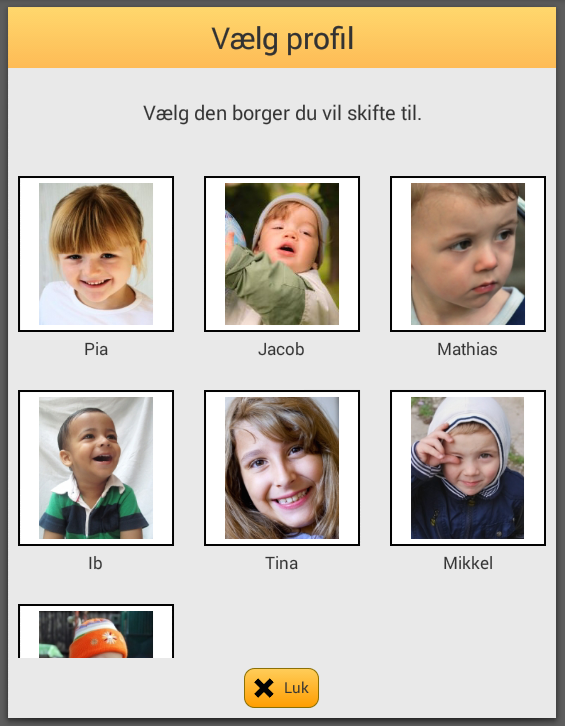
\includegraphics[scale=0.3]{dialog_profile_selector}
        \caption{Single profile selector}
        \label{fig:profile_selector_dialog}
    \end{subfigure}
    \hspace{5em}
    \begin{subfigure}[t]{0.4\textwidth}
    	\centering
        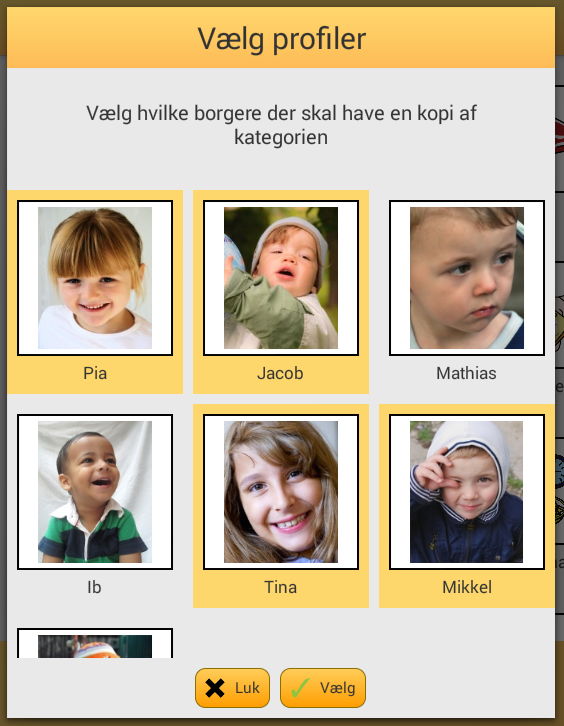
\includegraphics[scale=0.3]{dialog_profiles_selector}
        \caption{Multi profile selector}
        \label{fig:profiles_selector_dialog}
    \end{subfigure}
    
    \caption{Profile selectors}
    \label{fig:profile_selection}
\end{figure}

\section{Waiting Dialog}
\label{sec:waiting_dialog}

In cases where the system needs to peform some action that takes a long task (\secref{sub:long_tasks}, to indicate that the system is not frozen the waiting dialog, as it looks in \figref{fig:dialog_waiting}, can be used. \todo{refer to appendix}.

\begin{note}
	If one have temporally unused screen real estate at the location where one are conceptually loading in elements then you should place you progress bar or activity indicator in this unused screen real estate. A waiting dialog should only be used in the case when there are not enough screen estate awailable or in cases where it does not make sense to display a progressbar in the unused screen estate. An activiy indiactor as the progressbar should generally be used when there is no way of telling how long there will be til the task is complete. 
\end{note}


\begin{figure}[h]
	\centering
	
\includegraphics[width=0.4\textwidth]{dialog_waiting}
	\caption{Waiting dialog}
	\label{fig:dialog_waiting}
\end{figure}
\FloatBarrier

\subsection{Long Tasks}
\label{sub:long_tasks}
Long running tasks should generally not block the GUI. Any task that can potentially take a long time should be done on a background thread and NOT on the main GUI thread see \appref{app:threading_asynctask}. 

\section{Inflatable Dialog}
\label{sec:inflatable_dialog}

Some uses of dialogs might be more specific than the ones already existing in \gc, for this reason the inflatable dialog exists. If one wants to add input fields or a custom view one should use this dialog. In \figref{fig:inflatable_dialog}, an example of dialog is shown, this example shows the usecase when a user needs to edit a category.

\begin{figure}[h]
	\centering
	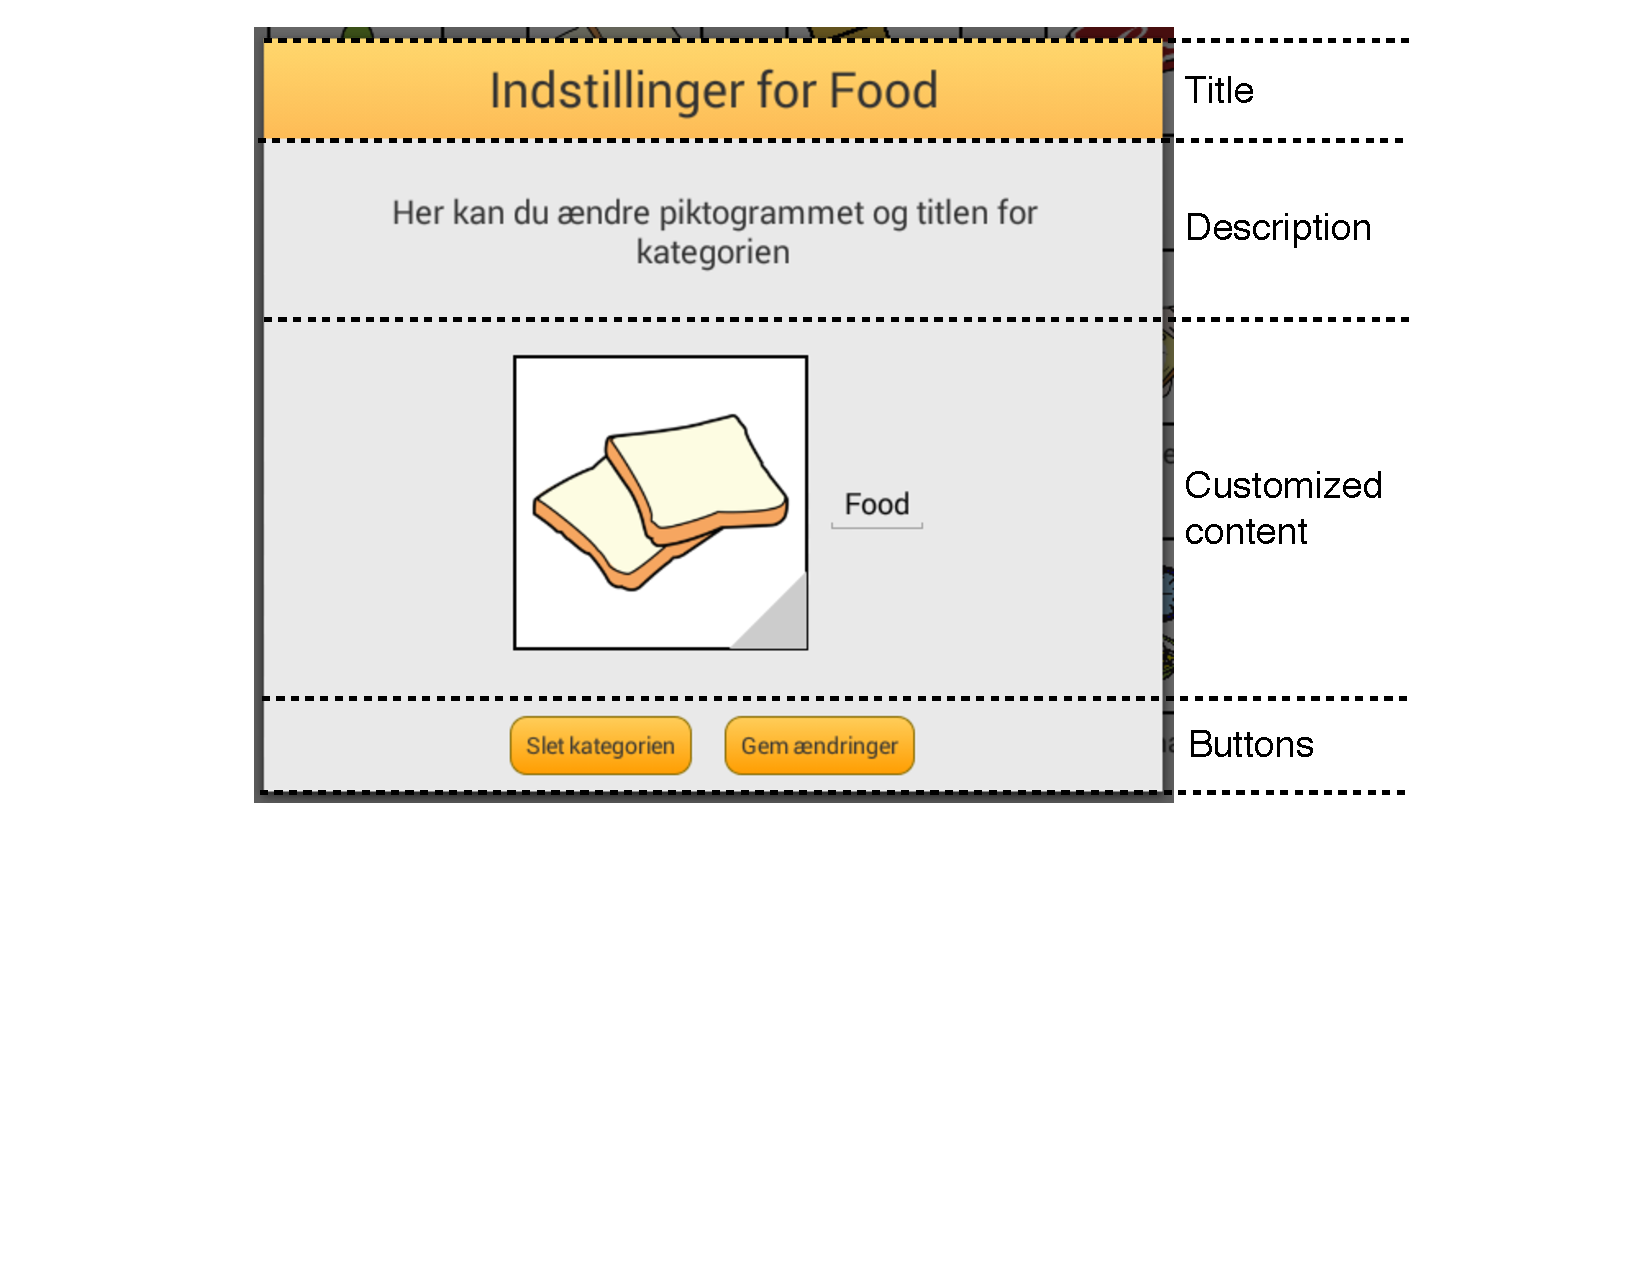
\includegraphics[width=0.6\textwidth]{dialog_inflatable}
	\caption{Inflatable dialog}
	\label{fig:inflatable_dialog}
\end{figure}
\FloatBarrier

\begin{note}
	It is important that if buttons should be added to this type of dialog it must be placed in the very bottom of the dialog and should be divided as shown in \figref{fig:inflatable_dialog}. Also note that buttons should be 40dp in height.
\end{note}





